% This version of CVPR template is provided by Ming-Ming Cheng.
% Please leave an issue if you found a bug:
% https://github.com/MCG-NKU/CVPR_Template.

%\documentclass[review]{cvpr}
\documentclass[final]{cvpr}

\usepackage{times}
\usepackage{epsfig}
\usepackage{graphicx}
\usepackage{amsmath}
\usepackage{amssymb}
\usepackage{float}
\usepackage{url}


% Include other packages here, before hyperref.

% If you comment hyperref and then uncomment it, you should delete
% egpaper.aux before re-running latex.  (Or just hit 'q' on the first latex
% run, let it finish, and you should be clear).
\usepackage[pagebackref=true,breaklinks=true,colorlinks,bookmarks=false]{hyperref}


\def\cvprPaperID{****} % *** Enter the CVPR Paper ID here
\def\confYear{CVPRW 2021}
%\setcounter{page}{4321} % For final version only
\pagenumbering{gobble}

\begin{document}

%%%%%%%%% TITLE
\title{A Deep Adversarial Framework for Visually Explainable Periocular Recognition}

\author{João Brito and Hugo Proen\c{c}a\\
IT: Instituto de Telecomunica\c{c}\~oes\\
 University of Beira Interior\\
 6200-001, Covilh\~a, Portugal\\
{\tt\small joao.pedro.brito@ubi.pt, hugomcp@di.ubi.pt}
}

\maketitle



%%%%%%%%% ABSTRACT
\begin{abstract}
   In the biometrics context, the ability to provide the reasoning behind a decision has been at the core of major research efforts. These explanations have powerful benefits, such as increasing trust amongst the users of a system and augmenting the system's overall accountability and transparency. In this work, we describe a periocular recognition framework that not only performs biometric recognition but also provides visual representations of the features/regions that supported a decision. Being particularly designed to explain non-match (''\emph{impostors}'') decisions, our solution uses adversarial generative techniques to synthesise a large set of ''\emph{genuine}'' image pairs, from where the most similar elements with respect to a query are retrieved. Then, assuming the alignment  between the query/retrieved pairs, the element-wise differences between the query and a weighted average of the retrieved elements yields a visual explanation of the regions in the query pair that \emph{would have to be different} to transform it into a ''\emph{genuine}'' pair. Our quantitative and qualitative experiments validate the proposed solution, yielding recognition rates that are similar to the state-of-the-art, but - most importantly - also providing the visual explanations for every decision. \footnotetext{\llap{\textsuperscript{*}}The code is publicly available at \url{ https://github.com/ojoaobrito/ExplainablePR.git}}
\end{abstract}

%%%%%%%%% BODY TEXT
\section{Introduction}

This work describes an integrated framework for periocular biometric recognition which - apart performing the recognition task - also provides a visual explanation that sustains every decision. Considering the biometric recognition ubiquity and dependability~\cite{demand_for_interpretability}, our main goal in this paper is not to propose a \emph{better} recognition framework in terms of the error rates, but to particularly diverge of the black-box paradigm and follow a \emph{visually explainable} paradigm, as illustrated in Fig. \ref{fig:interpretable_explanation}.

\begin{figure}[H]
  \begin{center}
  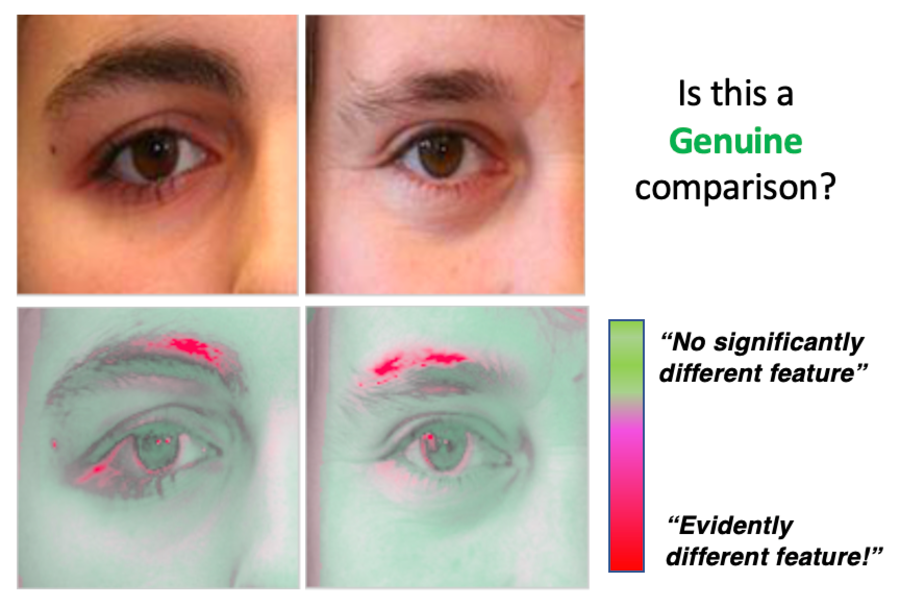
\includegraphics[width=0.47\textwidth]{figures/figure_1_nv2.pdf}
  \caption{Key insight of the proposed visual explainable framework:  given a pair of images, the system \textbf{not only reports a binary decision} (''\emph{genuine}''/''\emph{impostor}'' classes), but also \textbf{highlights the regions in each sample that contributed the most in case of a \emph{non-match} decision}. In this example, yet the iris and skin colour are similar between samples, the eyebrows and eyelashes shapes are evidently different, along with a skin spot in the sample illustrated at the left side. These are exactly the regions highlighted in the visual explanations.}
  \label{fig:interpretable_explanation}
  \end{center}
\end{figure}

Typically, a recognition problem involves a set of unique and non-transferable features that can unmistakably identify a subject. Biometric traits, as they are designated in the field, serve such purposes, as long as they are universal, distinguishable, resilient to changes and  easy to collect \cite{introduction_to_biometric_recognition}. Upon proving their compliance with these requirements, biometric traits can be divided into two major  categories: 

\begin{enumerate}
\item \textit{Physiological} features (e.g., the iris, fingerprint and retina) that are naturally possessed by a given subject; 
\item \textit{Behavioural} biometrics, that yield from the interaction between a subject and the surrounding environment (e.g., the gait and handwritten signature) \cite{biometric_recognition_dl_survey}.
\end{enumerate}


\begin{figure*}[h]
  \begin{center}
  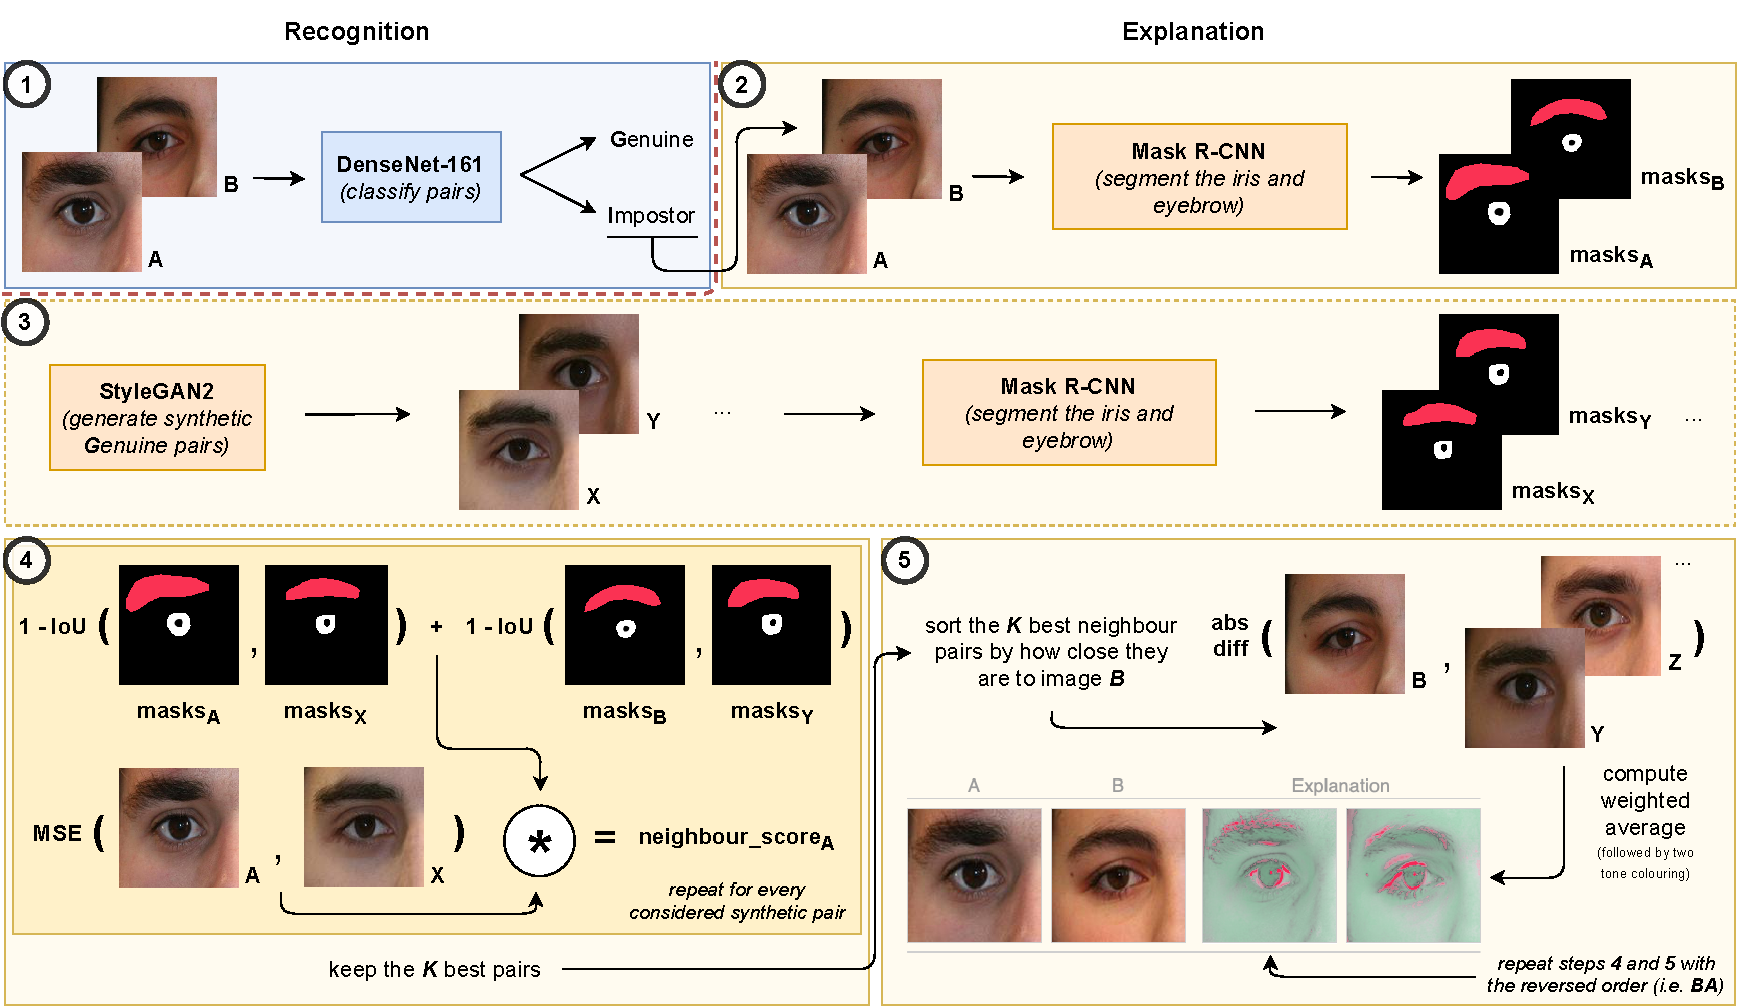
\includegraphics[width=0.97\textwidth]{figures/figure_2.pdf}
  \caption{Cohesive perspective of the main pipeline of the proposed solution. The first step (recognition) encompasses a CNN that distinguishes between ''\textit{genuine}'' and ''\emph{impostor}'' pairs. Then, upon an ''\emph{impostor}'' decision, steps two to five (explanation) find the $k$ ''\textit{genuine}'' synthetic pairs among a large set that most closely resemble the query pair. Assuming the alignment between the query and the retrieved pairs, the element-wise differences between the query and a weighted average of the retrieved elements provides a visual explanation of the regions/features in the query that would have to be different to turn the query into a ''\textit{genuine}'' pair.}
  \label{fig:main_diagram}
  \end{center}
\end{figure*}

Concentrating growing interests in the biometrics domain, periocular recognition uses the information in the vicinity of the eye to perform recognition, in which the iris, sclera, eyebrow, eyelid and skin stand out. 

Regarding the concept of \emph{explainability} and its application to recognition problems, it should be noted that Deep Learning solutions rely on model complexity and abstraction prowess to become truly accurate. Although seemingly innocuous, there could be seriously negative outcomes if such \emph{black-boxes} gamble on the clearance of unauthorised people into sensible areas. Hence, it is particularly important to provide human understandable explanations of the decisions, which will augment the overall system accountability and transparency, enabling a broader range of applications (i.e., forensics). Recently, the EU, through the GDPR \cite{gdpr}, introduced the notion of "\emph{right to an explanation}". Even though the definition and scope of such explanations are still subject to debate \cite{right_to_explanation}, these are definite strides towards a formal regulation regarding the importance given to the concept of explainability. \\

According to the above points, this paper describes a framework that receives a pair of images and returns a two-fold output: 1) a binary match/non-match decision, that discriminates between the ''\emph{genuine}''/''\emph{impostor}'' pairs; and 2) a \emph{visual explanation} that highlights the features/regions of the input data that sustained a particular decision. This is considered the main contribution of our work, in the sense that - to the best of our knowledge - it is the first that creates an accurate and explainable representation of the reasons behind certain decisions of the recognition system. Other contributions include the use of Generative Adversarial Networks (GANs), to synthesise visually pleasant images pair that faithfully resemble the distribution of the ''\emph{genuine}'' pairs, which augments the variety and flexibility  of the learning set and can be seen as an alternate form of data augmentation.

Fig. \ref{fig:main_diagram} provides a cohesive overview of the framework that performs the  recognition task and provides the corresponding explanations: at first, a CNN (of a well known architecture) is trained to discriminate between match/non-match decisions. If the pair is deemed to belong to the ''\emph{impostors}'' distribution, we find its most similar ''\emph{genuine}'' pairs in a large set of synthetic data. The insight here is that, even if the query pair has significant differences between its elements that led to an ''\emph{impostor}'' decision, the closest synthetic pairs most likely do not (as they were  drawn from the ''\emph{genuine}'' distribution). Then, assuming that the most likely synthetic pairs and the query are sufficiently aligned, obtaining the pixel-wise weighted differences between them will elevate visual disparities. \\

The remainder of this paper is organised as follows: Section \ref{sec:related_work} summarises the most relevant research  in the fields of periocular recognition and Machine Learning Explainability. Section \ref{sec:proposed_method} describes our method and Section \ref{sec:experiments_and_discussion} analyses the results obtained. Section \ref{sec:conclusions_and_further_work} concludes this paper, while also providing some final remarks.

%-------------------------------------------------------------------------

\section{Related Work}
\label{sec:related_work}

\subsection{Periocular Recognition}
\label{subsec:periocular_recognition}
The seminal breakthroughs in the periocular recognition problem can be traced to a set of methods termed \textit{feature descriptors}. Methods such as HoG, LBP and SIFT were able to produce simplified data representations by relying on edges, textures and keypoints, respectively. In \cite{feasibility_study}, the results from each feature descriptor were fused to faithfully discriminate between the ''\emph{genuine}''/''\emph{impostor}'' pairs. This work served as basis for subsequent fusion-based approaches, as in \cite{information_fusion_approach}.  In \cite{rbm_feature_learning} a Restricted Boltzmann Machine was used to learn a probabilistic distribution over the input data, further discriminated with metric learning and SVMs.

With the effective application of Deep Learning solutions, researchers turned to popular architectures (in particular Convolutional Neural Networks), to pursue ever increasing recognition accuracy. Accordingly, in \cite{accurate_periocular_recognition} the main concept involves the use of multiple CNNs that are specialised in classifying a particular kind of semantic information (e.g., gender or age). Then, a score fusion process yields the final response. In \cite{deep_prwis},  authors enforce a CNN to ignore the ocular region (due to its likelihood to contain specular reflections) and rely in the eye's surrounding area (eyebrow, eyelid and skin). \cite{person_identification} created independent representations of the iris and periocular regions, that feed classification modules, whose scores are finally fused to reach the decision. Using a multi-glance mechanism, where part of the intermediate components are configured to incorporate emphasis on the most important semantical regions (i.e., eyebrow and eye), Zhao and Kumar~\cite{zhao_kumar_novel} developed a recognition model that particularly focus these regions, enabling the deep Convolutional Neural Network (CNN) to learn additional discriminative features that improve the recognition capability of the whole model. Recently,  \cite{towards_interpretable_face_recognition} attempted to bridge the gap between biometric recognition and interpretability, by learning feature specific filters that respond to a range of preferred spatial locations. \cite{interpretability_by_parts} propose an integrated solution that leverages the discovery of parts as a form of attention. 

\subsection{Machine Learning Explainability}
\label{subsec:machine_learning_explainability}

In the literature, the existing explainable techniques are commonly divided in terms of their depth, scope and model applicability \cite{mythos_of_model_interpretability}, \cite{molnar2019}. Depth is related to the length to which we explain a given model, i.e., whether the technique limits the model's complexity to make it more transparent (\textit{intrinsic} explainability) or allows complexity and focuses on explaining exclusively the system outputs (\textit{post hoc} explainability). Scope indicates the range that a technique possesses, i.e., if it explains individual predictions (\textit{local}) or the model's entire behaviour (\textit{global}). Finally, applicability divides the techniques based on their model affinity, i.e., whether they are only compatible with a specific family of models (\textit{model-specific}) or any kind of model (\textit{model-agnostic}). The most commonly cited techniques include LIME \cite{lime} and Shapley codes (SHAP) \cite{shap}. The former uses a surrogate linear model, trained on perturbed data (e.g., disabled clusters of adjacent pixels), to locally approximate the behaviour of a complex black-box model. The latter uses game theory and Shapley values, which are assigned to the features based on how important they are to a given prediction. Additionally, Saliency Maps \cite{saliency_maps} use the derivative of a highly complex function (essentially, a CNN) with respect to a given input image, to determine which pixels need to be changed the least, while also changing the output class the most. Finally, for visualisation purposes and, therefore, outside the scope of this work, PDP \cite{pdp} and ALE \cite{ale} techniques are able to produce plots that correlate the independent variables to a target variable, exploiting the notions of marginal and conditional distributions, respectively.

%-------------------------------------------------------------------------

\section{Proposed Method}
\label{sec:proposed_method}

\subsection{Learning Phase}
\label{subsec:learning_phase}

The main components of the proposed method comprise three well known models: the DenseNet-161, Mask R-CNN and StyleGAN2. The first one (DenseNet-161) is trained to solve an identity verification problem, while the segmentation model (Mask R-CNN) is fine-tuned to produce high-quality masks for the iris and eyebrow. Finally, the GAN model (StyleGAN2) learns how to create synthetic data that, while closely resembling the distributions in the training set, is diverse enough to approximate unseen subjects. Additionally, a fourth, auxiliary model (ResNet-18) is fitted to discriminate between images from the left and right sides of the face. Although trained separately, all the models learn from the same training split, which excludes a set of disjoint IDs that are reserved for performance evaluation purposes.

Regarding the model used in the verification task (DenseNet-161), it should be stated that it has much more parameters than the network used by Zhao and Kumar~\cite{accurate_periocular_recognition} in their solution. This might be the fact that sustained slightly better recognition performance of our model with respect to the baseline (Sec. \ref{subsec:quantitative_evaluation}), but also at the expense of a substantial higher computational cost of classification than the baseline, which might be impracticable in some cases.

\subsection{Inference Phase}
\label{subsec:inference}

Once trained, our method is conceptually divided into five major steps, as depicted in Fig. \ref{fig:main_diagram}. Firstly, the DenseNet-161 model is used to verify the claimed identity: upon receiving a pair of images, the model discriminates  between ''\emph{genuine}''/''\emph{impostor}'' pairs. If the pair is deemed to be ''\emph{impostor}'', the remaining steps create a visually interpretable explanation of that decision.

The second step takes the query pair and, using Mask R-CNN, segments the irises and eyebrows regions. Next, step three uses the StyleGAN2 generator to create a large, synthetic set of exclusively ''\emph{genuine}'' pairs (i.e., where both images belong to the same person). For each of these synthetic pairs, the ResNet-18 model determines its side configuration (i.e., whether images regard the left or right side of the face) and, as before, masks are obtained by the segmentation model. 

After obtaining the synthetic data and their corresponding masks, the synthetic dataset is indexed based on the coordinates of the center of the iris, which will enable faster search in the retrieval step. To that end, the clustering algorithm K-Means is trained on a subset of the iris segmentation masks to obtain three centroids, one for each major iris gaze family (i.e., left, centre and right). This way, we index the available pairs based on their combination of iris positions (e.g., left-left, right-centre \ldots). By doing so, when searching, we can just rely on the synthetic pairs that share the same combination as the test pair, saving time and useless calculations. 

Upon settling for a portion of the synthetic dataset that closely meets the iris position constraint, the segmentation masks are further used to determine which synthetic pairs have the iris and eyebrow approximately overlapped to the query. This is an important requirement to obtain visually pleasant explanations, given that pixel-wise differences are extremely sensitive to differences in phase (i.e., component misalignment). Accordingly, we obtain a similarity score $s_X$ between each synthetic neighbour and the query using:
\begin{equation}
    s_X = \omega_{\text{masks}} * ||\text{query}_{\text{A}} - \text{neighbour}_{\text{X}}||_2,
\label{eq:neighbour_score}
\end{equation}
being $||.||_2$ the $\ell-2$ norm and $\omega_.$ a weight that considers component misalignment. This way, we obtain a weighted distance between each synthetic neighbour and the first image of the query pair. $\omega_{\text{masks}}$ values serve to favour pairs that have good alignment, considering $1 - \text{IoU}(.,.)$, i.e., the complement of the intersection-over-union of the synthetic/query segmentation masks. In practice, we search amongst the (large) thousands of synthetic pairs, the closest to the query pair in terms of the first image. Therefore, given that the second image of the query pair is from a different subject, it will most likely have features that are different to the synthetic neighbours, which are exactly the kind of dissimilarities that make up the final explanations.

This way, the $k$ closest neighbours are sorted according to their element-wise distance to image $B$, using  (\ref{eq:neighbour_score}). Finally, to produce the final explanation, the $k$ best neighbours are used to obtain the pixel-wise differences against the query pair image $B$. In practice, a neighbour distance is subtracted from the total sum of distances, creating an inverted distance. This assures that the contribution of the closest synthetic neighbours to the final result is more important than of those with bigger distances. 

\subsection{Implementation Details}
\label{subsec:implementation_details}
The DenseNet-161 model was trained for $15$ epochs with a learning rate of $0.0002$ and a batch size of $64$ image pairs. The Adam algorithm was used for the weight optimisation process (with default $\beta_1$ and $\beta_2$ values). A similar training setup was used to train the ResNet-18 model, albeit for a smaller number of epochs (i.e., $5$).
For the Mask R-CNN's training process, we kept its default values, using a learning rate of $0.001$, a batch size of $1$ and $30$ epochs worth of training (in this case, fine-tuning from the COCO pre-trained weights).
Regarding the StyleGAN2 architecture, the used training step comprised a total of $80000$ iterations and a batch size of $8$. After converging, the generator is capable of synthesising realistic looking images, such as the roughly $400000$ pairs that make up the artificial dataset. Finally, for the number $k$, that determines how many synthetic pairs should be kept, we used a default value of $15$.


%-------------------------------------------------------------------------

\section{Experiments and Discussion}
\label{sec:experiments_and_discussion}

\subsection{Datasets and Working Scenario}
\label{subsec:datasets}
As mentioned above, the proposed framework is composed of two modules: 1) one for recognition; and 2) the other for explanation purposes. Regarding the former, the chosen CNN is solely trained on the UBIPr dataset \cite{ubipr}, which provides the ID annotations used in the identity verification problem. Regarding the explanation step, it mainly relies on a combination of UBIPr and FFHQ \cite{stylegan}. Despite not being directly applicable to the context of this work (i.e., it contains full face images, thus requiring extra steps to extract the periocular region), the FFHQ dataset contains a large variety in terms of periocular attributes, some of which are scarcer in the UBIPr dataset. In practice, a small, but curated, portion of the FFHQ samples was used to create a data super set. Regardless of their source, all images were resized to a common shape, depending on the task (i.e., 512x512x3 for Mask R-CNN, 256x256x3 for StyleGAN2 and 128x128x3 for the CNNs).

 As it is usual in the biometric recognition context, it is important to define proper working modes and world settings, for which the system is built. With respect to the working mode, our model runs in verification mode (also referred to as \textit{one-to-one}), where the system validates a claimed identity~\cite{introduction_to_biometric_recognition}. As for the world setting, we assume an open-world setting, meaning that unseen subjects can be faithfully handled in the inference step.
 
 \begin{figure*}
  \begin{center}
  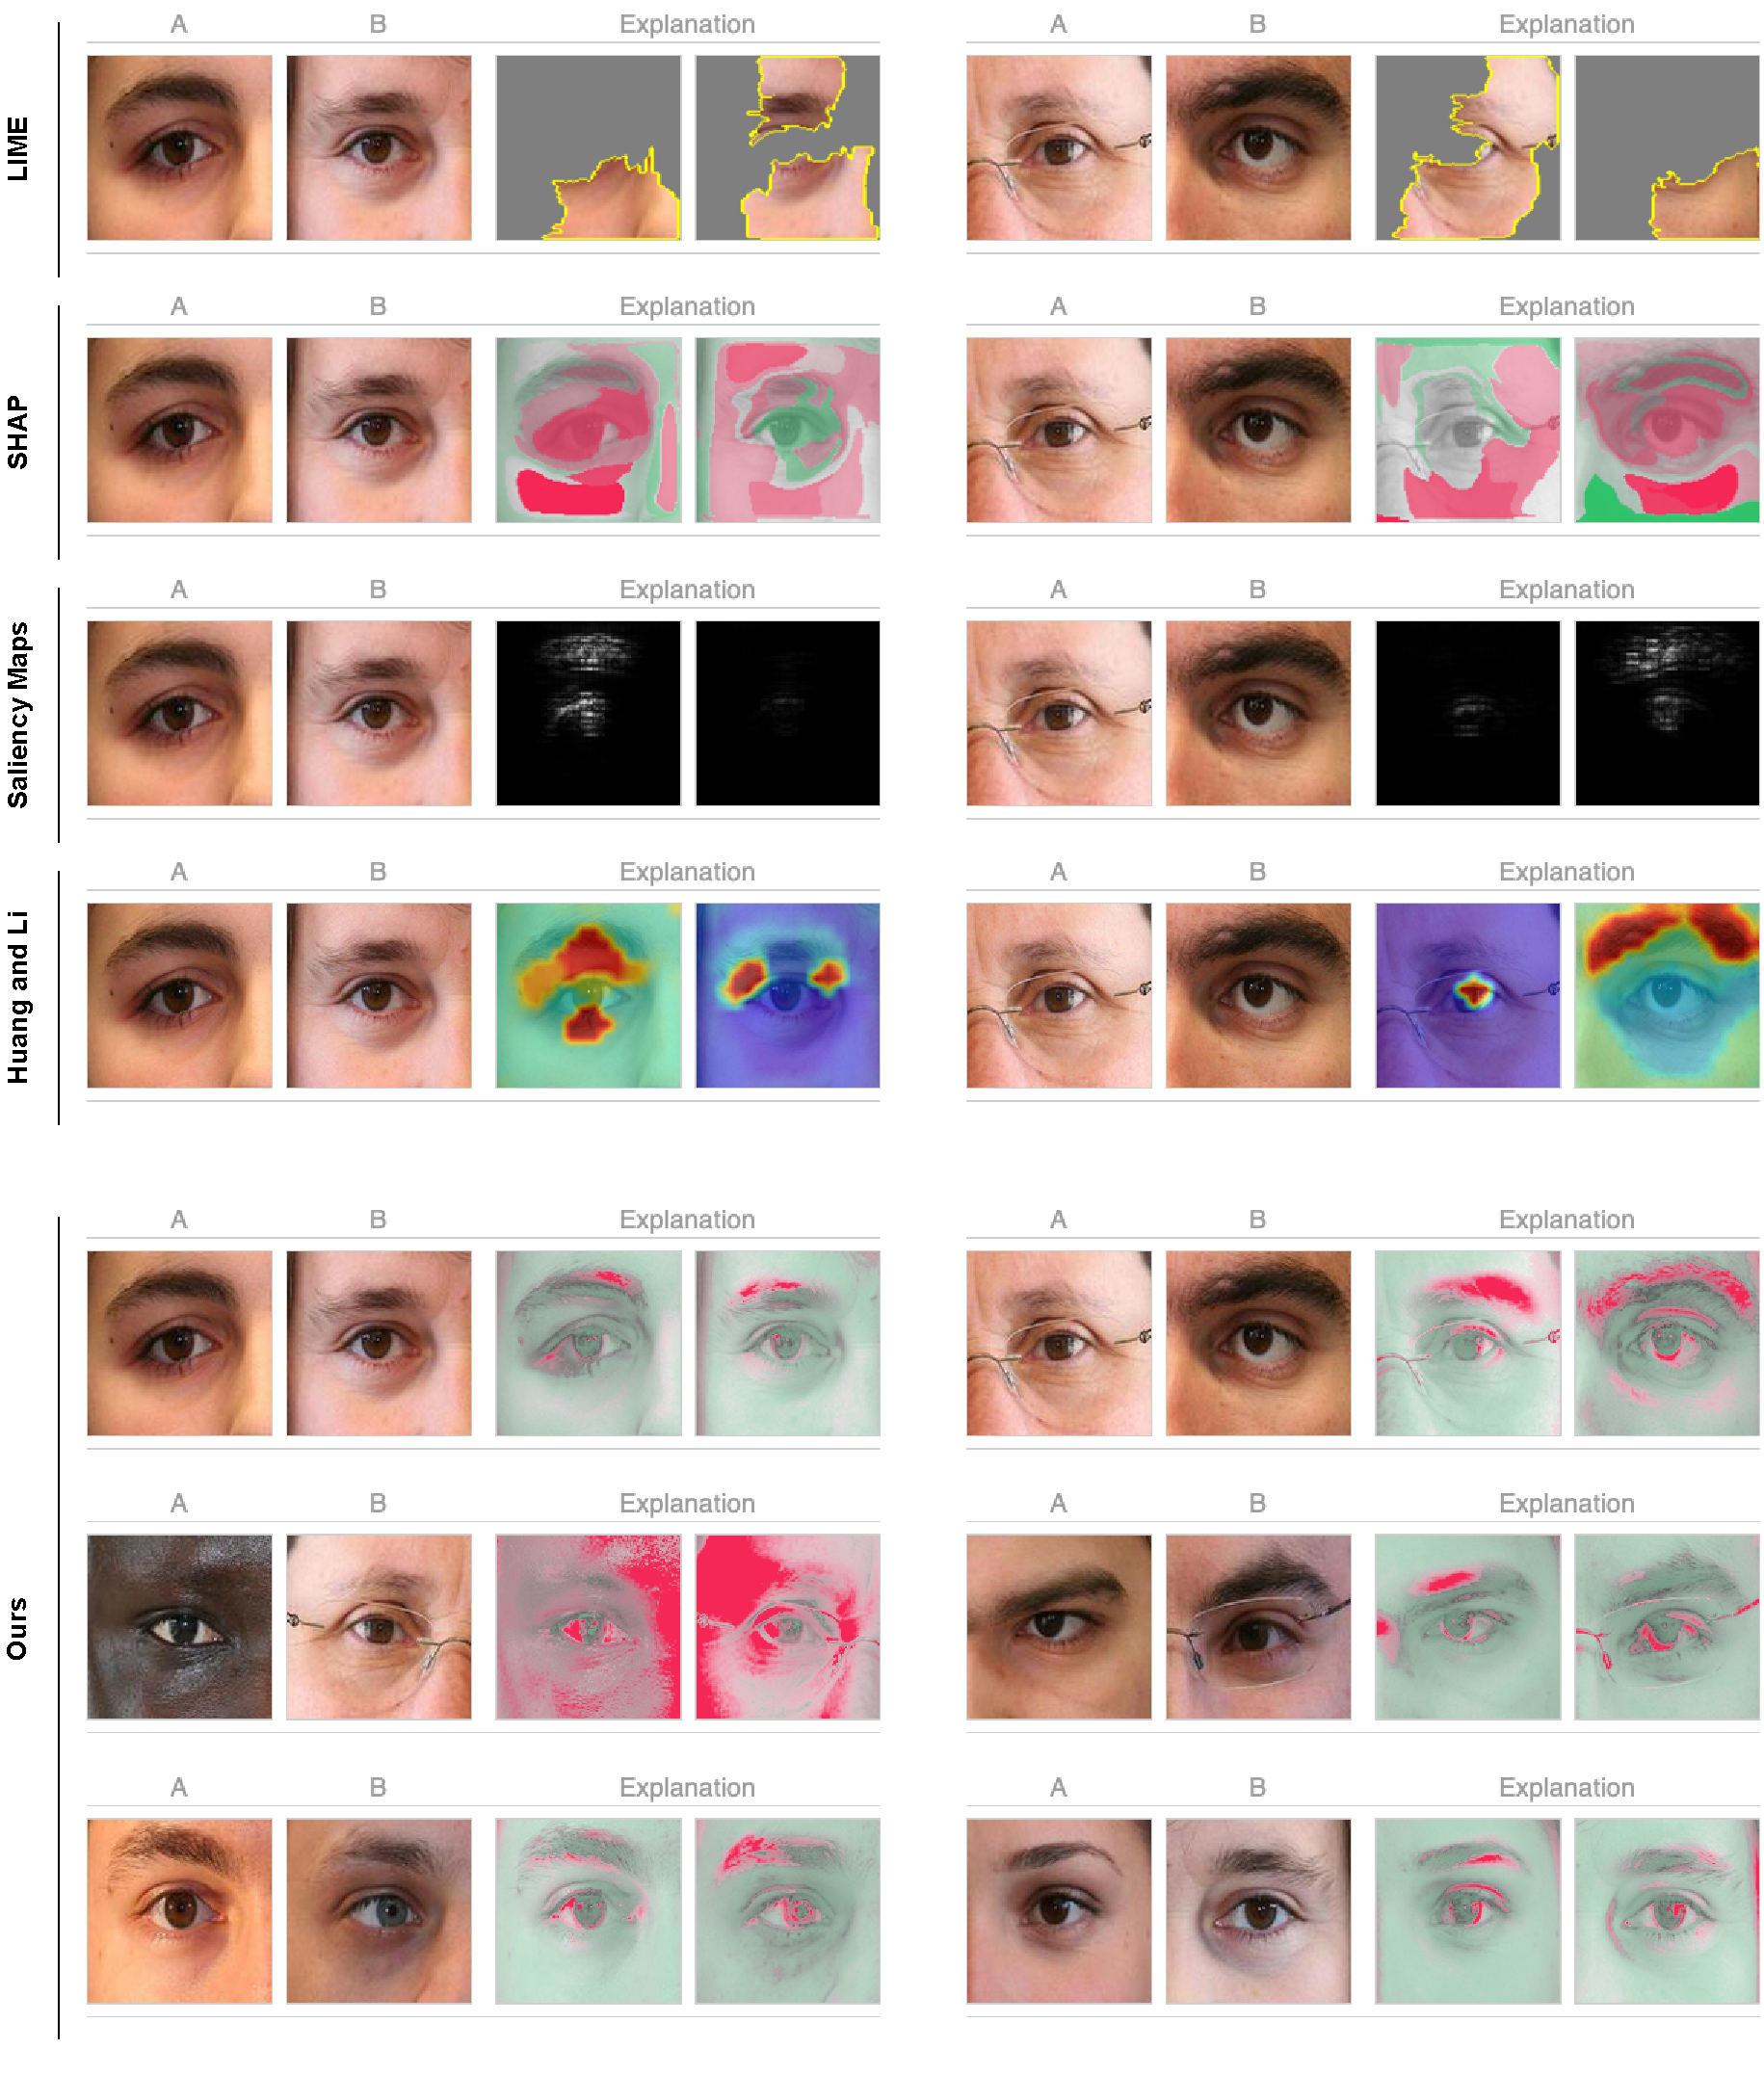
\includegraphics[width=\textwidth]{figures/figure_4.pdf}
  \caption{Examples of the results attained by three standard interpretability techniques (LIME, SHAP and Saliency Maps), a state-of-the-art interpretable deep model for fine-grained visual recognition (i.e., \cite{interpretability_by_parts}) and our method. Notice how our results are clearer in highlighting the components that justify every non-match decision (e.g., skin texture and color, eyebrows/eyelashes size and distribution, irises color and even skin spots).}
  \label{fig:results}
  \end{center}
\end{figure*}

\subsection{Explainability Evaluation}
\label{subsec:qualitative_evaluation}

 Our explainability chain starts by the train of a DenseNet-121 model to perform the verification task. This model can be further paired to either LIME, SHAP or Saliency Maps to create comprehensive comparison schemes, to which we add the method described in \cite{interpretability_by_parts}. 
Fig.~\ref{fig_synthetic} provides several examples of the synthetic ''\emph{genuine}'' images pairs generated from the GAN model. Apart their obvious visual realism, it is important that this set contains samples with the most likely known data covariates for the periocular region: varying gazes, wide-opened/closed eyes, varying poses, partial occlusions, and even varying facial expressions. Failing in incorporating such diversity will determine that the closets synthetic pairs of a query will still be notoriously different from it, and that the visual representations obtained will have poor realism.  

 \begin{figure}
  \begin{center}
  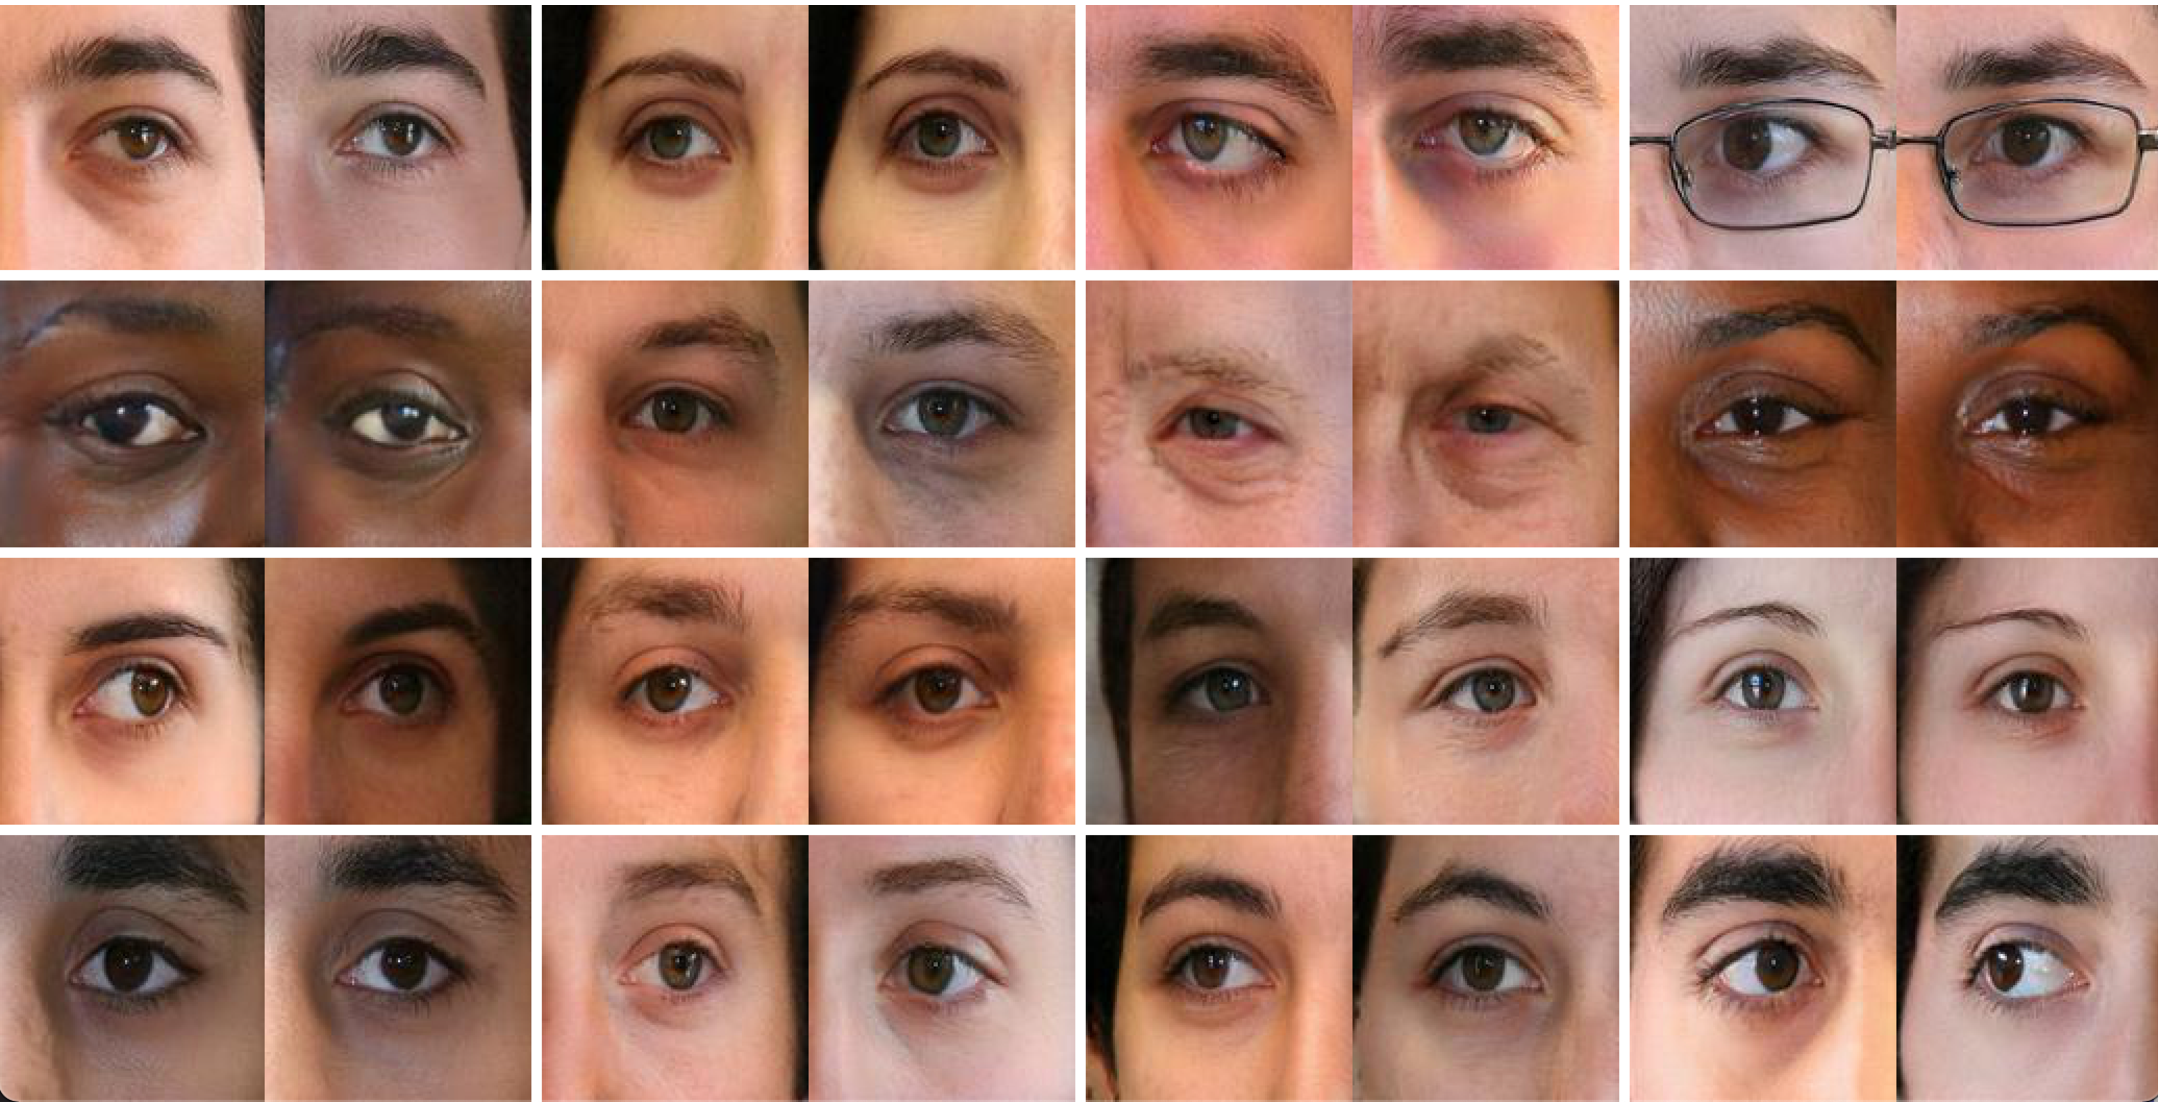
\includegraphics[width=225pt]{figures/images_GANs.pdf}
  \caption{Examples of the synthetic image pairs in our dataset, generated according to a GAN model. These elements are drawn exclusively from the \emph''{genuine}'' distribution. Upon  a query, the most similar synthetic pairs with respect to the query are found, which will provide the features/regions that would transform the query into a ''\emph{genuine}'' comparison.}
  \label{fig_synthetic}
  \end{center}
\end{figure}


Fig. \ref{fig:results} displays the expected results from a visually explainable system. In practice, LIME tries to keep the most important super-pixels, SHAP highlights those it deems important in red tones and Saliency Maps produce greyscale explanations. As for the method by Huang and Li, it generates a heat-map in which red tones elevate important areas. Focusing on the common pairs between all methods, the left sample is essentially different with regards to eyebrow thickness and presence/absence of a noticeable skin spot. As for the right one, the most obvious disparities have to do with the eyebrow areas. Overall, our results are the most informative, when compared with the remaining four solutions. While LIME and SHAP do a decent job, Saliency Maps provide a faint explanation. It is Huang and Li's method that comes closer to our level of visual appeal, by clearly highlighting portions of the eyebrow and a portion of subject $A$'s skin spot, in the left pair. Moreover, when given the right sample, it generates a solid red area comprising subject $B$'s eyebrow. However, upon closer inspection, our results show more appealing visual cues: in the left sample, distinct red tones on top of $A$'s skin spot and eyelashes, as well as, reiterated eyebrow differences in the right sample with highlights in both eyebrows, rather than just one. As for the remaining samples, the third (just below the first) is clearly explained by highlighting the entirety of both skin areas, which are obviously different between images $A$ and $B$. Finally, in the fourth pair it is also shown how the eyelids differ, by colouring that periocular component on subject $B$'s image, and, in the fifth sample, subjects $B$'s eyebrow and iris are accurately shown in red.

When objectively measuring the differences between the explanations provided by the proposed method and the baselines (LIME, SHAP, Huang and Li (HL) and  Saliency Maps (SM)), we used a set of $10$ heterogeneous test queries and measured the pixel-wise explanation coefficients returned by each technique, which correspond to the importance (weight) given by each method to a particular image position for a decision. Next, considering that any meaningful correlations between the responses of two methods would have to be linear, we measured the Pearson's linear correlation between pairs of techniques:

\begin{equation}
    r_{xy} = \frac{\sum_i (x_i - \hat{x}) (y_i -\hat{y})}{\sqrt{\sum_i (x_i -\hat{x})^2 \sum_i (y_i -\hat{y})^2}},
\label{eq:neighbour_score}
\end{equation}
where $x_i/y_i$ denote the i$^{th}$ scores provided by each technique and the $\hat{.}$ symbol denotes the mean value. This way, $r_{xy}$ measures the similarity between explanations provided by the $x$ and $y$ techniques: values close to $0$ will correspond to more independent explanations, while values towards $1$ will hint at semantic similarities between such explanations.

 \begin{figure}
  \begin{center}
  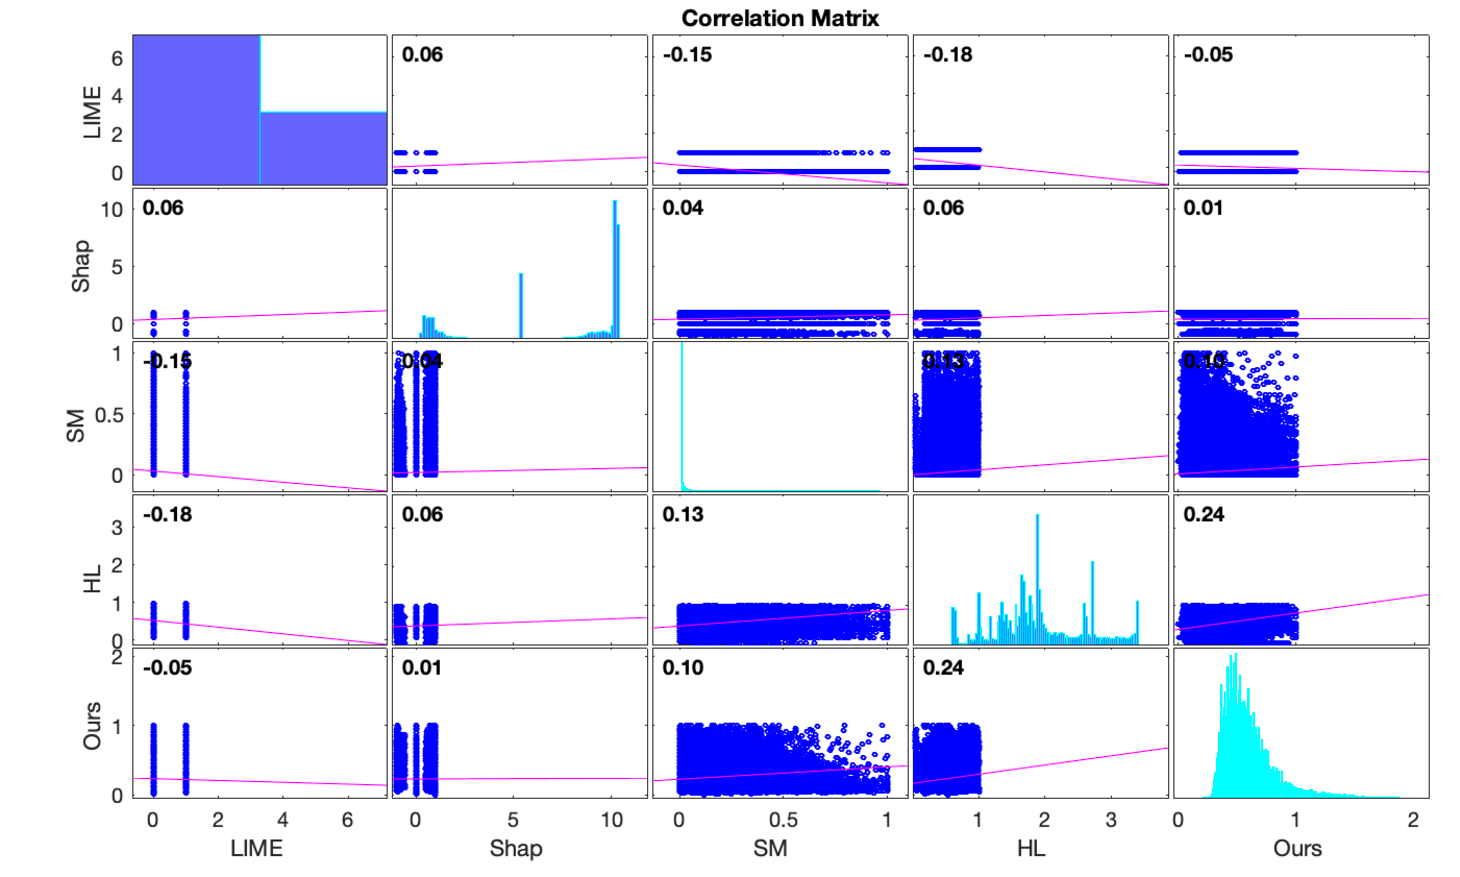
\includegraphics[width=233pt]{figures/correlation.pdf}
  \caption{Pearson correlation values between the pixel-wise responses provided by the method proposed in this paper (Ours) and four baselines techniques (LIME, SHAP, Huang and Li (HL) and  Saliency Maps (SM)).}
  \label{fig:correlation}
  \end{center}
\end{figure}

The results are provided in the confusion matrices shown at Fig.~\ref{fig:correlation}, where the main diagonal provides the distributions of the scores generated by each technique and the remaining cells provide the scatter plots between pairs of techniques with the Pearson's correlation value $r_{xy}$ given at the top left corner of each cell ('SM' stand for Saliency Maps and 'HL' denotes the Huang and Li solution)). All these techniques report a local numeric value that corresponds to the role/importance of each region in the final decision. The exception is LIME, where the pixels are binary discriminated into ''visible''/''occluded'. In this case, we considered that ''visible'' will be equal to 1, while 'occluded'' will be equal to 0. Overall, we observed that the techniques provide relatively independent responses for the importance given to each pixel in the final decision. Interestingly, in some cases, there are even negative correlation values between two methods (e.g., HL and LIME or SM and LIME). There are other pairs of solutions that achieved almost full independence between their responses (the Shapley/Ours methods), which points for completely different strategies being used to define the explaining regions/features. Still considering our method, its levels of correlation were kept relatively low with respect to the remaining methodologies, achieving values of  0.24 with respect to the method of Huang and Li (the most correlated), and 0.1 for Saliency maps. Still, we concluded that the proposed solution is extracting  semantic information (e.g., features and regions) of the vicinity of the human eye that is evidently different of the kind of information emphasised  by any of the remaining methods, which supports the usefulness of the solution described in this paper.

\subsection{Recognition Accuracy Evaluation}
\label{subsec:quantitative_evaluation}

At first, note that we do not aim at providing a \emph{better} recognition framework than the state-of-the-art, in terms of the recognition rates.  Even though, our main purpose in this section was to perceive if the proposed recognition/explanation network is able to achieve competitive recognition performance with respect to state-of-the-art implementations.

We compare the recognition effectiveness of the proposed method with respect to a well known periocular recognition model (due to Zhao and Kumar~\cite{accurate_periocular_recognition},  considered to represent the state-of-the-art). Using the UBIRIs.v2 set \cite{ubiris_v2} and the learning/evaluation protocols described in~\cite{accurate_periocular_recognition}, we obtained the results summarised in Table \ref{tab:quantitative_evaluation}. Also, we provide  ROC values of the proposed strategy, that can be fairly combined with the similar ROC plot provided by the original authors of the baseline in~\cite{zhao_kumar_novel}.

A bootstrapping-like strategy was used, by sampling 90\% of the available data in UBIRIS.v2 and dividing the resulting samples between two disjoint sets: 80\% for training and the remaining 20\% for test. The models were trained separately in each sample and the performance evaluated in the corresponding test set, from where the EER and AUC scores were obtained. This process was repeated 10 times, to perceive the mean $\pm$ standard deviation values for both metrics. Overall, results were satisfactory, particularly considering that - due to our modular design - the recognition module of the proposed framework can be easily replaced by any other, while keeping its explainability abilities.

\begin{table}[!h]
\small
{\renewcommand{\arraystretch}{1.5}%
\begin{center}
 \begin{tabular}{|c | c | c|} 
 \hline
 \textbf{Method} & \textbf{EER} & \textbf{AUC} \\
 \hline
 \hline
 Ours (open-world) & $0.108 \pm 3\mathrm{e}{-2}$ & $0.813 \pm 5\mathrm{e}{-2}$ \\
 Ours (closed-world) & $\mathbf{0.087 \pm 2\mathrm{e}{-2}}$ & $\mathbf{0.910 \pm 2\mathrm{e}{-2}}$ \\
 Zhao and Kumar \cite{accurate_periocular_recognition} & $0.109 \pm 2\mathrm{e}{-3}$ & $-$ \\[1.5pt]
 \hline
\end{tabular}
\end{center}}
\caption{Comparison between the recognition rates attained by the proposed method (in both world settings) and a state-of-the-art method (strictly operating in an open-world setting). Results are given for the same learning/test sets of the UBIRIS.v2 dataset.}
\label{tab:quantitative_evaluation}
\end{table}

For reference purposes, Fig.~\ref{fig:ROCs} provides the Receiver Operating Characteristic (ROC) curve for our solution. When comparing to the corresponding results reported by authors in~\cite{accurate_periocular_recognition} in the same set, a close recognition summary performance between both methods can be derived (as seen in Table~\ref{tab:quantitative_evaluation}). Overall, we observed a similar performance between these techniques in this dataset, supporting the idea that our solution is able to approach state-of-the-art recognition rates.

\begin{figure}[h]
  \begin{center}
  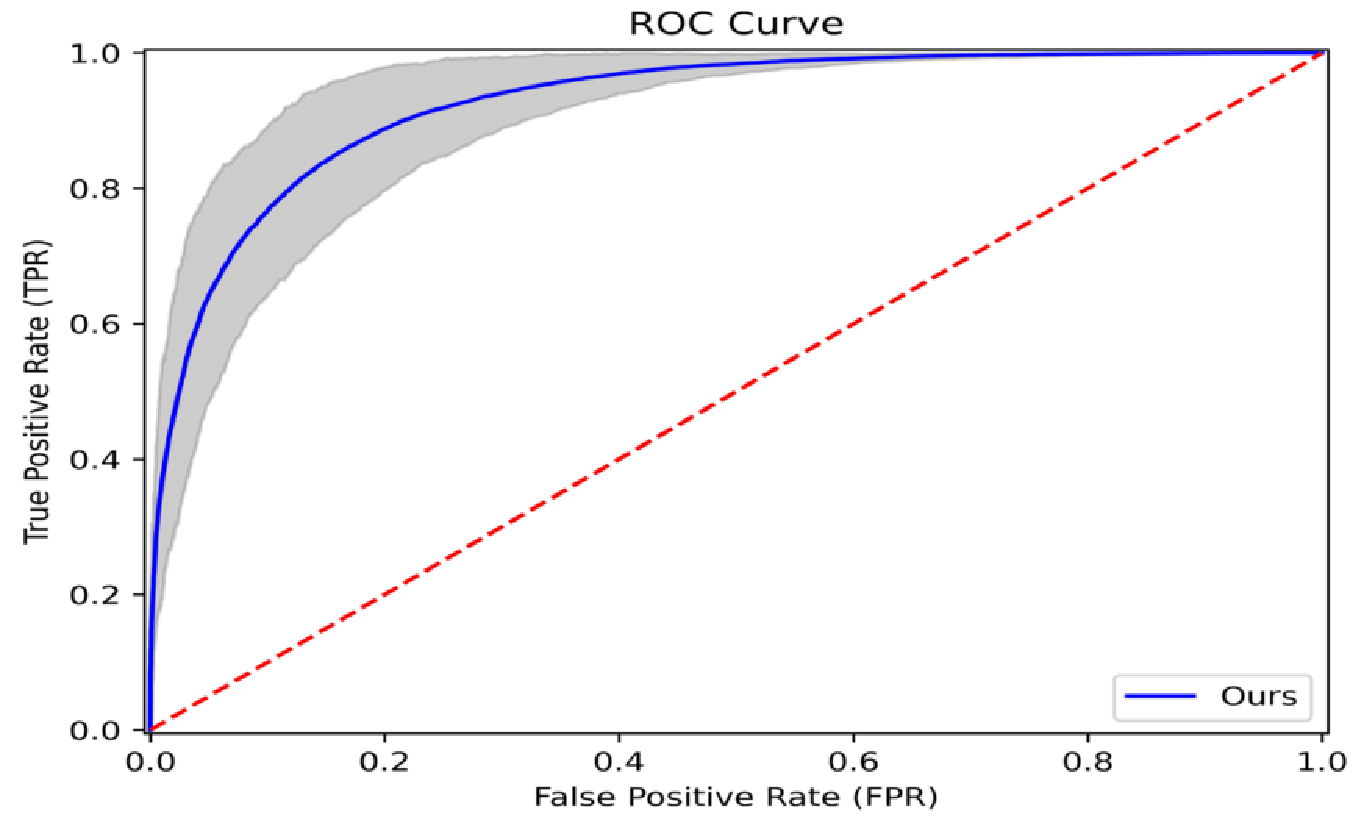
\includegraphics[width=250pt]{figures/ROCs.pdf}
  \caption{Receiver Operating Characteristic (ROC) curve obtained for the proposed method, using the UBIRIS.v2 set and a similar empirical protocol as Zhao and Kumar~\cite{accurate_periocular_recognition}. The ROC curve equates to EER and AUC values of 0.108 and 0.813, respectively.}
  \label{fig:ROCs}
  \end{center}
\end{figure}

% width = 0.25\textwidth for the vertical image
% width = 0.47\textwidth for the horizontal image

\begin{figure}[h]
  \begin{center}
  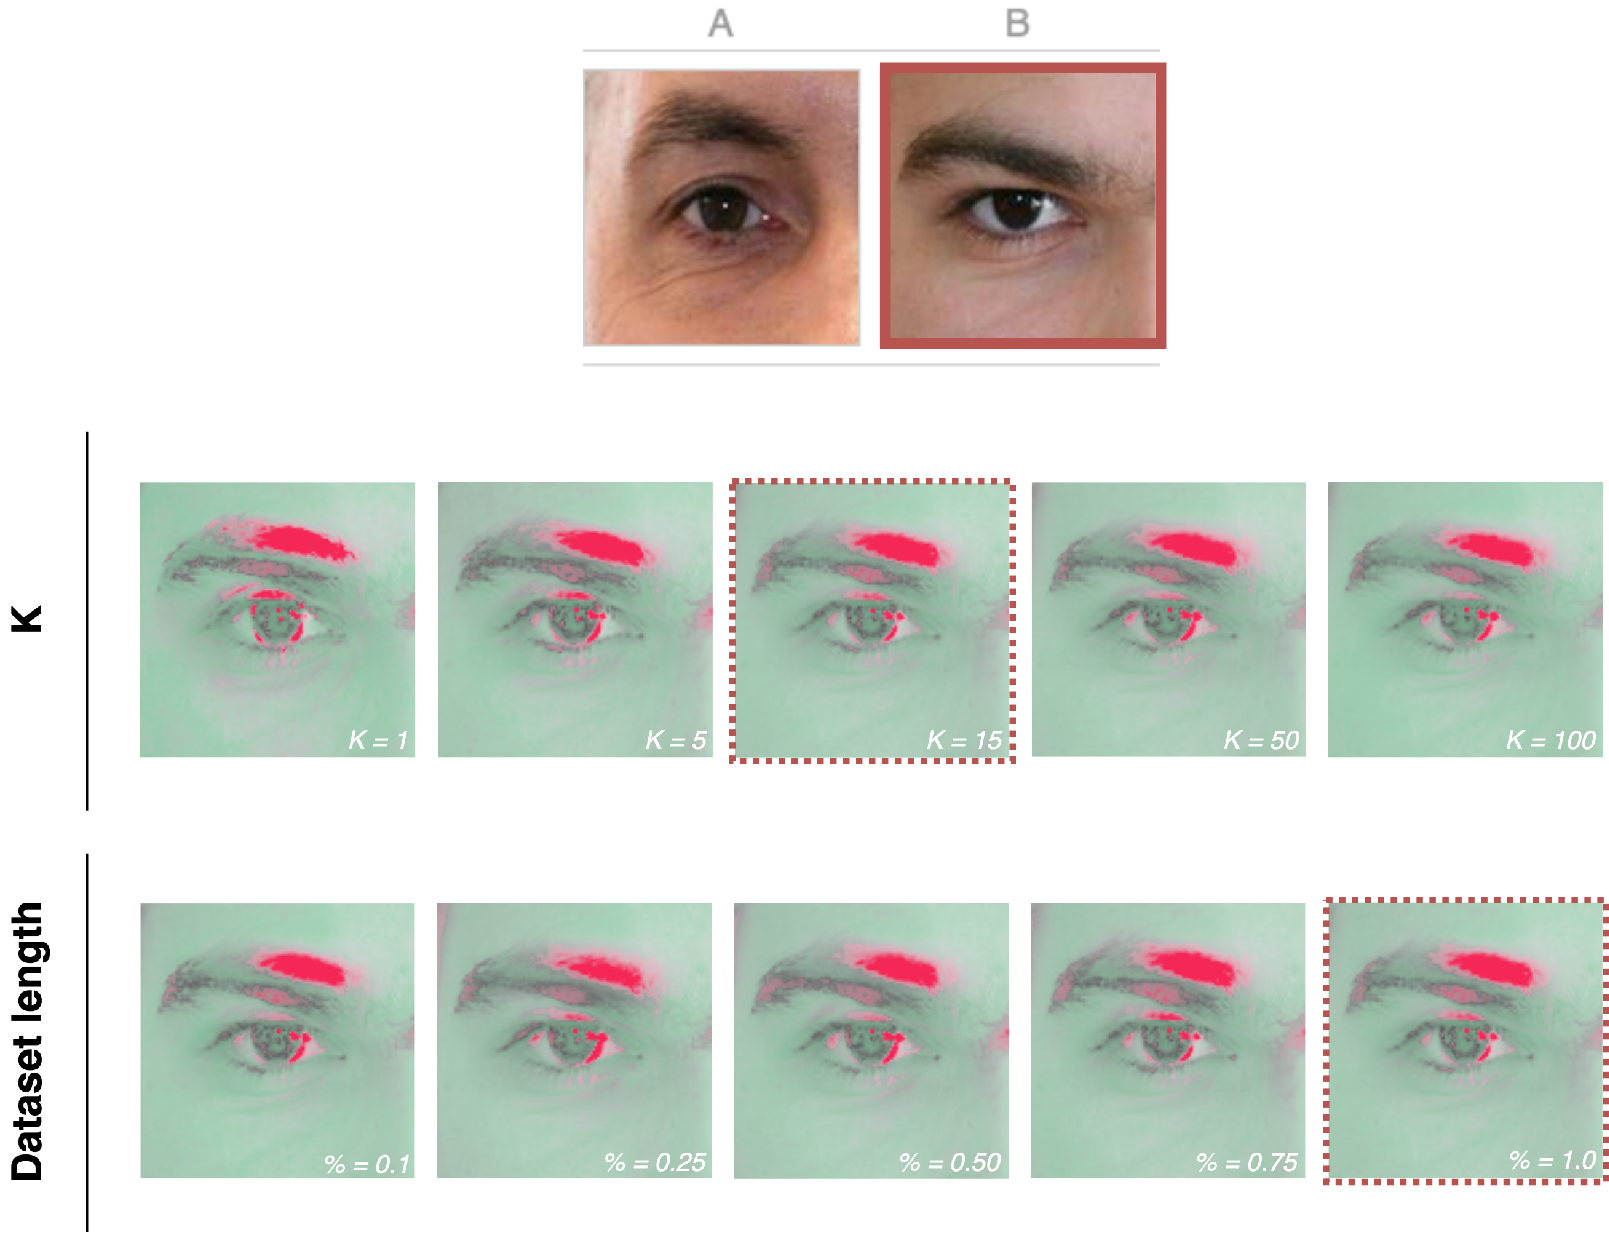
\includegraphics[width=0.47\textwidth]{cvpr2021AuthorKit/latex/figures/figure_5_horizontal.pdf}
  \caption{Typical changes in the results when two key parameters of the proposed method are varied. The red square indicates which image is being \emph{explained} (i.e., $B$), while the red dashed squares provide the default values used. In general, increasing $k$ up to $15$ allows for smoother explanations, as does keeping a large dataset. Reducing the latter tends to produce less sensitive results, substantially decreasing the plausibility of the explanations generated.}
  \label{fig:ablation_study}
  \end{center}
\end{figure}

\subsection{Ablation Studies}
\label{subsec:ablation_study}
For our ablation experiments, we identified two hyper-parameters of our method that might play the most significant roles in the final effectiveness of the whole solution: 1) the number of neighbours retrieved ($k$) from the synthetic set for every query and 2) the length of the synthetic set itself. This section discusses how changes in these values affect the quality of the generated explanations in a less than optimal way (as seen in Fig. \ref{fig:ablation_study}).

\subsubsection{Number of Neighbours}
\label{subsubsec:number_of_closest_neighbours}
The value $k$ determines how many synthetic pairs are considered with respect to a query. Overall, we observed that smaller values lead to more sensitive and jagged results. Up to a certain point (e.g., $15$), increasing $k$ typically enables to obtain \emph{smoother} explanations, due to the larger number of samples taken into account when averaging the closest neighbours. This trend, however, starts returning incremental improvements (notice in Fig. \ref{fig:ablation_study}, where $k\geq50$  progressively stops presenting a prominent tone on the eyelid).

\subsubsection{Length of the Synthetic Dataset}
\label{subsubsec:synthetic_dataset_length}

This is the most sensitive parameter of our solution. Considering that it is important to find ''\emph{genuine}'' pairs that closely resemble a query, it is particularly sensitive to assure that all typical periocular data variations are faithfully represented in the synthetic set, assuring that the retrieved elements (i.e., the most similar) will have its major components (iris, eyebrows and eyelids) aligned to the query itself. If this condition is not satisfied, the explanations loose their biological plausibility and effectiveness.
Fig. \ref{fig:ablation_study} illustrates how smaller synthetic sets lead to less evident explanations, especially around the eyelid and the eyebrow. 

%-------------------------------------------------------------------------

\section{Conclusions and Further Work}
\label{sec:conclusions_and_further_work}
This paper described an integrated framework, based in well known deep-learning architectures, to simultaneously perform periocular recognition and - most importantly - to provide visual explanations of the regions/features that sustained every \emph{non-match} decision, which we consider to be the cases where explanations are the most required. According to the powerful generative ability of GANs, we create a very large set of synthetic pairs that follow the ''\emph{genuine} distribution''. At inference time, for every ''\emph{impostor}'' comparison we are able to perceive the regions and features that \emph{failed the most} (i.e., those that most evidently were different from a subset of the ''\emph{genuine}'' synthetic pairs). This enables to generate pleasant explanations, where each component of the target region appears with a different colour depending on how it influenced the final decision. Importantly, the modular nature of our method ensures that the periocular region can be replaced by other biometric traits (e.g., the face) without compromising the explanations. 

As future work, we are developing a strategy for also providing intuitive explanations of the ''\emph{genuine}'' observations, where the strategy has to be very different from the idea behind the ''\emph{impostors}'' insight used in this paper.

\section*{Acknowledgements}
This work is funded by FCT/MEC through national funds and co-funded by FEDER - PT2020 partnership agreement under the project UIDB//50008/2020. Also, it was supported by operation Centro-01-0145-FEDER-000019 - C4 - Centro de Compet\^encias em Cloud Computing, co-funded by the European Regional Development Fund (ERDF) through the Programa Operacional Regional do Centro (Centro 2020), in the scope of the Sistema de Apoio \´a Investiga\ç{c}̧\~{a}o Cient\´ifica e Tecnologica - Programas Integrados de IC\&DT.

{\small
\bibliographystyle{ieee_fullname}
\bibliography{egbib}
}

\end{document}
